% Checked with grammarly
\chapter{Data Generation Framework}
\label{sec:benchmark}
In this chapter, the framework and its components are described: error types (Section~\ref{sec:error_types}), data and error generation (Section~\ref{sec:data_gen}), and validation of the results (Section~\ref{sec:validation}).
Unlike other frameworks discussed in Section~\ref{sec:background}, this framework uses only clean and dirty versions of real datasets to scale them up while maintaining data characteristics, without taking any additional hand-crafted input or constraints.

% Checked with grammarly
\section{Types of Errors}
\label{sec:error_types}

Data errors are values that differ from the ground truth.
In this context, we differentiate between data with and without errors by calling it clean or dirty. 
Completely clean data is ground truth (GT).  


In the context of this benchmark, we have a clean ground-truth dataset and a dirty version with introduced errors.  
Leveraging this, faulty values can be found by locating the cells that differ between dirty and clean. 
This information is helpful to detect errors and their distribution, and frequencies of specific values being error prone.  
Moreover, it is useful for classification of error types.


\textbf{Five error types}, that are common in the real-world datasets, are considered in this benchmark: 
Missing values, typos, outliers, replacements and swaps. 
The error types and descriptions are shown in Table~\ref{tab:generator_errors}.


\textbf{Missing value} is the simplest type of error that is frequently seen in our experimentation. 
Generally, there are three sub categories of missing values: 
Missing Completely at Random (MCAR), Missing at Random (MAR), Missing Not at Random (MNAR). 
MCAR is a value that is missing completely independently from other values. 
Missing values have no dependencies or ties to any other values in the dataset. 
MAR occurs when the missing value is random, but is related to the part of the observed data, an instance of this is where in datasets with personal weight, females are less inclined to include their weight. 
MNAR means that the missing value of an observation depends on its values, for instance, using the weight example again, weight is not reported for obese individuals.
MNAR analysis is problematic because the distribution of the missing observations depends on both observed and unobserved values.
Missing data introduce various problems. 
First, the absence of data reduces statistical power of the dirty dataset, moving it's statistical properties further from ground truth.
Second, the lost data can cause bias in the estimation of parameters. The previous example of people not reporting if they are obese could be a cause of this. 
Third, the representativeness of the samples can influence the set of distinct values, frequencies, and ratios between them.


The benchmark supports MCAR and MAR. 
% TODO how we maintain these properties


\textbf{Typo} is a typographical error that typically is introduced by misspelling. 
Common instances of typos are \textsc{Morrocco} and \textsc{Lost Angeles}. 
Introducing typos can violate the set of distinct values, since new distinct values can be inserted.
This can be detrimental for techniques such as one-hot-encoding that is highly sensitive to the number of distinct values.
In the benchmark, the typo distribution and the distinct value set are used to estimate the number of new unique typos to add to the generated output. 
The new distinct typos are generated by modifying existing values. Modifications are controlled by measuring Levenshtein distance between the clean and modified values. 


\textbf{Outlier} is a data point that significantly differs from a data distribution.
An example of this could be human adult height equal to 3m, 20cm, or a negative value such as -1.5m. 
Since outliers increase variability in data, they decrease statistical power.
In our benchmark we are introducing outliers while preserving dirty data statistics. 
New outlier values are created using correction, in Equation~\ref{eq:outlier_correction}. 
Correction is used to shift actual mean of the data to the desired dirty mean. 
To introduce outliers preserving the statistics, every new outlier should be balanced by another outlier. 
% TODO
Thus, we generate outlier value and it is mirroring such that
we need to set up maximal distance to we reflect upper and lower limits that define outliers  
\begin{equation}
\label{eq:outlier_correction}
\textsc{correction} = \frac{(\textsc{mean\_dirty} - \textsc{mean\_generated}) \cdot \textsc{nrow\_generated})}{\textsc{num\_outliers}}
\end{equation}
% TODO other explanation how we limit outlier with correction

% # Recompute limits for later balancing: max distance to mean, holds for both sides
%         dist_from_mean_to_outliers = max(abs(upper_limit - err_dist.dirty_mean[col_name]), abs(err_dist.dirty_mean[col_name] - lower_limit))
%         lower_limit, upper_limit = err_dist.clean_mean[col_name] - dist_from_mean_to_outliers, err_dist.clean_mean[col_name] + dist_from_mean_to_outliers

%         # Reflect around zero and subtract correction
%         distance_to_zero = max(abs(lower_limit), abs(upper_limit))
%         lower_limit, upper_limit = (-1 * distance_to_zero) - correction, distance_to_zero - correction

\textbf{Replacement} is a flipped value that was chosen from the existing set of valid values. 
For example, in feature with distinct set of values \textsc{\{A, B, C\}}, \textsc{A} can be replaced by \textsc{D}. 
Replacement does not introduce new distinct values, but change the frequencies of the different distinct values. 
This reduces statistical power of the dirty dataset, moving it's statistical properties further from ground truth.
In the benchmark, to preserve statistical properties, pairs of correspondences of replacements are detected and scaled randomly. 

\textbf{Swap} is a pair of values swapped between two columns: numerical and categorical, categorical and categorical or two categorical.
% TODO




The focus is on a single source datasets, thus multiple data source datasets and errors that occur during schema integration are not considered.


Data errors can be categorized by levels of their appearance in the data: single value, within a single feature, within a single tuple, within several features or tuples.

% TODO bias
% TODO in-estimation

% Our error generation includes properties such as:
% \begin{itemize}
%     \item Error type: A variety of different error types can be introduced to the data.
%     \item Error rate: A configurable for each error rate, that specifies am amount of occurances of respective error.
%     \item Reproducibility: Each and every introduced error can be reproduced and tracked.
% \end{itemize}


% \begin{table}[!h]
% \caption{\label{tab:generator_errors}Errors preserved by generator}
% \begin{tabular}{l|l|l}
% \toprule
% Error name    & Parameters                                                                                                             & Description                                                                           \\ 
% \midrule
% Missing value & \begin{tabular}[c]{@{}l@{}}text text text text text text \\ text text text text text text\end{tabular} & \begin{tabular}[c]{@{}l@{}}text text text text text text \\ text text text text text text\end{tabular} \\
% Typo          &\begin{tabular}[c]{@{}l@{}}text text text text text text \\ text text text text text text\end{tabular} & \begin{tabular}[c]{@{}l@{}}text text text text text text \\ text text text text text text\end{tabular} \\
% Outlier       &\begin{tabular}[c]{@{}l@{}}text text text text text text \\ text text text text text text\end{tabular} & \begin{tabular}[c]{@{}l@{}}text text text text text text \\ text text text text text text\end{tabular} \\
% Replacement   &\begin{tabular}[c]{@{}l@{}}text text text text text text \\ text text text text text text\end{tabular} & \begin{tabular}[c]{@{}l@{}}text text text text text text \\ text text text text text text\end{tabular} \\
% Swap          &\begin{tabular}[c]{@{}l@{}}text text text text text text \\ text text text text text text\end{tabular} & \begin{tabular}[c]{@{}l@{}}text text text text text text \\ text text text text text text\end{tabular} \\
% \bottomrule
% \end{tabular}
% \end{table}
\section{Data Generation}
\label{sec:data_gen}
For this framework we introduced two implementations to generate scaled up datasets: Local and distributed.
Both implementations maintain data and error statistics. 
The framework contains full pipelines consisting of the following generalized steps:

\begin{itemize}
    \item Read clean and dirty data.
    \item Data analysis and error classification.
    \item Scale up clean data.
    \item Generate errors and introduce to clean.
    \item Save generated dirty dataset.
    \item Generated data analysis.
\end{itemize}

\subsection{Local Data Generation}
\label{sec:local_generator}
\tikzset{bb/.style={draw, inner sep=2.5mm, rounded corners}}
\tikzset{
    ultra thin/.style= {line width=0.1pt},
    very thin/.style=  {line width=0.2pt},
    thin/.style=       {line width=0.4pt},
    semithick/.style=  {line width=0.6pt},
    thick/.style=      {line width=0.8pt},
    very thick/.style= {line width=1.2pt},
    ultra thick/.style={line width=1.6pt}
}

\begin{figure}
    \centering
    
    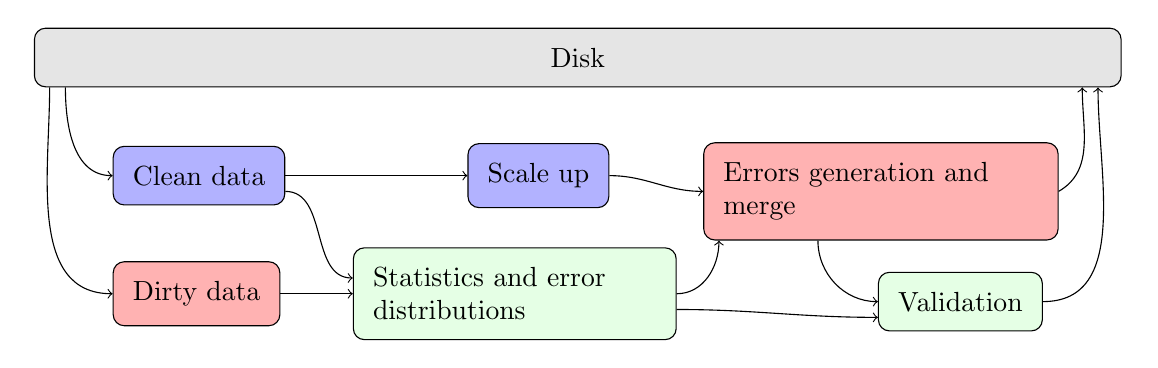
\begin{tikzpicture}[]
    \node[bb, text width=13.3cm, align = center, fill=black!10](disk){Disk};
    
    \node[bb, anchor = west, fill=blue!30] (clean) at ([yshift=-1.5cm, xshift = 1cm] disk.west) {Clean data};
    \node[bb, anchor = west, fill=red!30] (dirty) at ([yshift=-3cm, xshift = 1cm] disk.west) {Dirty data};
    
    \node[bb, text width=3.6cm, fill=green!10] (stats) at ([yshift=-3.0cm, xshift = -0.8cm] disk) {Statistics and error distributions};
    
    \node[bb, fill=blue!30] (scale_up) at ([yshift=-1.5cm, xshift = -0.5cm] disk) {Scale up};
    
    \node[bb, fill=red!30, text width=4.0cm, anchor = east] (errors) at ([yshift=-1.7cm,xshift= -0.8cm] disk.east) {Errors generation and merge};
    
    \node[bb,  anchor=east, fill=green!10] (validation) at ([yshift=-3.1cm, xshift=-1cm] disk.east) {Validation};
    
    \draw[->] ([xshift=0.4cm]disk.south west) to[out = -90, in = 180] (clean);
    \draw[->] ([xshift=0.2cm]disk.south west) to[out = -90, in = 180] (dirty);
    
    \draw[->] ([]clean.east) to[out = 0, in = 180] (scale_up);
    
    \draw[->] ([yshift=-0.2cm]clean.east) to[out = 0, in = 180] ([yshift=0.2cm] stats.west);
    
    \draw[->] ([]dirty.east) to[out = 0, in = 180] (stats);
    
    \draw[->] ([]scale_up.east) to[out = 0, in = 180] (errors);
    
    \draw[->] ([]stats.east) to[out = 0, in = -90] ([xshift=0.2cm]errors.south west);
    
    \draw[->] ([]errors.east) to[out = 30, in = -90] ([xshift=-0.5cm]disk.south east);
    
    \draw[->] ([]validation.east) to[out = 0, in = -90] ([xshift=-0.3cm]disk.south east);
    
    \draw[->] ([xshift=-0.8cm]errors.south) to[out = -90, in = 180] ([]validation.west);
    
    \draw[->] ([yshift=-0.2cm]stats.east) to[out = 0, in = 180] ([yshift=-0.2cm]validation.west);
    
    \end{tikzpicture}
    
    \caption{\label{fig:data_gen_local}Local data generator}
\end{figure}

First, for scaling to in-memory sizes there is a local data generator execution that consists of the following steps that are also shown in Figure~\ref{fig:data_gen_local}:

\textbf{Read:} 
Reading of clean and dirty datasets is done via Pandas DataFrames. 
Pandas is chosen for its' flexibility, large API and ease of coding. 
An important part of the reading is detecting a schema.
Pandas has a schema detection that allows reading dirty data while handling features with different data types. 
Python in general supports collections are allowed to contain heterogeneous data types. 
These properties together allow creation of a save schema for the dirty data.
But the automatic schema detection is not always precise, and integer cases can be detected as floats. 
Therefore, for the clean data, custom schema detection is applied. A sample of the data is extracted and analysed for fine-grained data types. 

\textbf{Error analysis:} 
Error analysis is performed on the clean and dirty datasets together.
First, distinct values of actual data are aggregated, and a binary difference mask of clean and dirty datasets is created.
The mask allows the framework to know the ratio and exact number of errors introduced in each feature, and to track detected and undetected errors. 
Errors are analyzed in a particular sequence, since if cell was classified as error of one type, it can not contain any other error types, this is based on the simplifying assumption that there are no compound errors.
First, missing values are detected using the Pandas \textsc{isnull()} method. 
Second, outliers are detected by interquartile range (IQR), shown in Formula~\ref{eq:is_outlier_iqr}, and by distribution, shown in Formula~\ref{eq:is_outlier_std}. 
Formula~\ref{eq:is_outlier_iqr} uses IQR, Formula~\ref{eq:outlier_iqr}, to define lower and upper limits, while Formula~\ref{eq:is_outlier_std} relies on standard deviation, Formula~\ref{eq:std}. 
Lower and upper limits are saved, and then reused during error generation. 
Third, dirty data is inspected for replacements. 
Replacements are cells that differ from the clean dataset, but still belong to a clean distinct values set.
Fourth, to find swaps between features, the framework computes row sums utilizing the binary difference mask. 
For rows with more than 2 errors, faulty cells are checked for swaps using an all-pairs comparison of dirty cells with clean values. 
For easiness during error generation, swaps are divided into numerical (between 2 numerical features) and mixed (between string and any other feature), since swaps between string and numerical features violate schema integrity.
Finally, all remaining erroneous \emph{string} feature values are classified as a typo.

\begin{equation}
\label{eq:outlier_iqr}
\textsc{IQR} = \textsc{Q}(0.75) - \textsc{Q}(0.25)  
\end{equation}

\begin{equation}
\label{eq:is_outlier_iqr}
\textsc{IQRO}(v) =  v < \textsc{Q}(0.25) - 1.5 \cdot \textsc{IQR} \ \cap \  v >  \textsc{Q}(0.75) + 1.5 \cdot \textsc{IQR}
\end{equation}

\begin{equation}
    \label{eq:std}
    \textsc{STD}(a) = \sqrt{\overline{|a - \overline{a}|^2}} 
\end{equation}

\begin{equation}
\label{eq:is_outlier_std}
\textsc{STDO(v)} = v < \overline{a} - 3 \cdot \textsc{STD} \ \cap \ v > \overline{a} + 3 \cdot \textsc{STD} 
\end{equation}

\textbf{Analysis of statistical properties:} 
Statistics analysis is performed by computation of univariate statistics such as min, max, mean, variance, kurtosis and skeweness are computed for both clean and dirty datasets.
When scaling the dataset, the framework strives towards maintaining these statistics at two steps.
First, when scaling the clean dataset, the statistics of the clean dataset are maintained. 
Second, when introducing errors, the detected errors and their distribution are preserved.
To reflect a realistic dataset, Schlosser~\cite{HassNSS1995} and Hasso Stokes~\cite{HassS1998} distinct item estimators are used. 
The dirty dataset is used as a sample of the generated. It is assumed that depending on the distribution of the distinct errors in the dirty dataset, more or a equivalent number of distinct values are introduced when scaling the data.

\textbf{Scaling up:} 
Scaling up clean data while preserving statistics is challenging, especially if applied at random. 
For instance, in a column with all unique values, the probability of selecting all values at least once is low when scaling factor is small. 
It is similar to the rolling dice with 6 unique sides. 
Scaling to 2x is equivalent to rolling 6 unique sides at least once with 12 trials.
To avoid this inconsistency, it was chosen to scale up by replication. 
If the scaling factor is greater is a floating point number, then the integer part is replicated, and the remaining floating part is sampled randomly from the clean data.

\textbf{Error generation and introduction:} 
Error generation and introduction is done column wise. 
Since the main workload of the framework is in this phase, each column is processed in parallel, with the exception of multi column errors such as swaps.
Typos, missing values and replacements are added to the scaled dataset in the first iteration.
For missing values and typos the distinct items sets and frequencies are gathered from the error analysis and statistics phases. 
Existing missing values and typos frequencies are scaled by scaling factor. Additionally, a specific number of new unique values is generated, this number is estimated as described in Scaling up.
The number of occurrences of a new unseen unique value is computed similar to n-gram smoothing techniques. 
The new frequency of unseen values is defined by Laplace smoothing "add-one" to avoid the zero-frequency problem.
The zero-frequency problem: If an individual class label is missing, then the frequency-based probability estimate will be zero.
To introduce the errors into the data, a vector with shuffled random indices is allocated and then utilized. 
For each unique error type a slice of indices is extracted and then apply to the scaled dataset.
Replacements are added using earlier created dictionaries of original and replaced values, and their frequencies.
Cells to modify are filtered, then a sub-fraction is randomly sampled and corrupted.
Since replacements do not introduce new distinct items, no additional computations are necessary. 
Similarly, swaps are done by filtering two columns and randomly choosing rows to exchange. 
The number of rows to modify is computed from the original number of swaps and scaling factor.
The last step is the addition of outliers. 
They are applied at the end of the sequence because, if applied correctly, they can scale the mean of the new scaled dataset to the desired dirty mean through the technique described in Section~\ref{sec:error_types}. 


\textbf{Write:}  
The freshly generated dataset is saved immediately after the error generation. It is written to the disk in comma-separated values (CSV) format. 
Dataset is saved before validation to ensure that we have the generated data, even if validation fails or concludes invalid generation.


\textbf{Validation:} 
The last stage of the framework is validation of generated dataset. It is done by comparing the statistics of the original dirty and generated datasets, the details are described in Section~\ref{sec:validation}.
The error distribution of the generated dataset is stored while generating and introducing the errors.
The univariate statistics are computed after the full generation is finished.
Both univariate statistics and error distribution are used for the validation. 
Additionally, all statistics are saved to files.

\textbf{Limitations of the local execution:} 
The Pandas DatFrames are relatively slow. Pandas is written C, and switching between C and Python takes time, especially for mathematical computations and data retrieval.
Another limitation is the in-memory computation. This means that data can not scale above aggregated memory of a single machine.
Third, there is potential for more parallelization of different parts of the local execution. But the parts already parallelized include the critical parts.


\subsection{Distributed Data Generation}
\label{sec:distributed_generator}

The distributed generator is for scaling to larger sizes of data that can not fit local memory restrictions.
It consists of the following steps that are also shown in Figure~\ref{fig:data_gen_dist}:

\textbf{Read:} 
Reading of clean and dirty datasets is similar to local execution. 
To compute statistics and detect schema, local Pandas DataFrames are used. 
On the other hand, the lazily evaluated Spark DataFrame is defined for further scaling up.
The schema applied to the Spark DataFrame is obtained from a schema detection of the dirty data in Spark.
This is important to avoid schema violations while introducing different from data types into clean feature.  
For instance, swaps can be introduced between numerical and string columns.

\textbf{Error analysis and statistics: } This step is equivalent to the local.

\textbf{Distributed scaling up:}
Scaling of the dataset in distributed mode is achieved via three different phases. 
Since Spark DataFrame is not indexed per default, to scale it up, one of the possibilities is to append DataFrame to itself, similarly to the local.
But because of Spark usability and API, it is possible to avoid concatenation by using a combination of Spark user-defined function (\textsc{UDF}) and \textsc{explode}.
First, we define a column with sequential indices. 
Then, this column is used by a \textsc{UDF} to map each existing row index to a list of new sequential row indices.
Finally, Spark \textsc{explode} utilizes these lists to "explode" (replicate) rows with a new index.

\textbf{Error generation:} 
Erroneous values are generated locally using error characteristics collected from the original dirty dataset.
The values are combined with row indices to create new error locations.
Indices are chosen at random for missing values, typos and outliers, or based on the filtering of specific values for replacements and swaps.
A challenging part here is to guarantee that indices are non-intersecting. 
To achieve this property, replacements are performed first, and afterwards random indices for other errors are chosen, avoiding already used indices.
This process is parallelized to write buffered strings of error tuples to HDFS, materializing and persisting the errors introduced in the scaled dataset.
These files can also be seen as meta data.
Introducing the errors into the actual distributed scaled up dataset is done by reading errors into Spark DataFrame from HDFS, and joining it on synthetic index.

\textbf{Write to HFDS:} 
Writing to HDFS was initially done using csv format, similar to the local data generation.
However, utilizing Spark compression and parquet format reduced runtime significantly.

\textbf{Validation:}  
Results validation same to local, except Spark functions are used to aggregate statistics for comparison of the generated and original dirty datasets.
\tikzset{bb/.style={draw, inner sep=2.5mm, rounded corners}}
\tikzset{
    ultra thin/.style= {line width=0.1pt},
    very thin/.style=  {line width=0.2pt},
    thin/.style=       {line width=0.4pt},
    semithick/.style=  {line width=0.6pt},
    thick/.style=      {line width=0.8pt},
    very thick/.style= {line width=1.2pt},
    ultra thick/.style={line width=1.6pt}
}

\begin{figure}
    \centering
    
    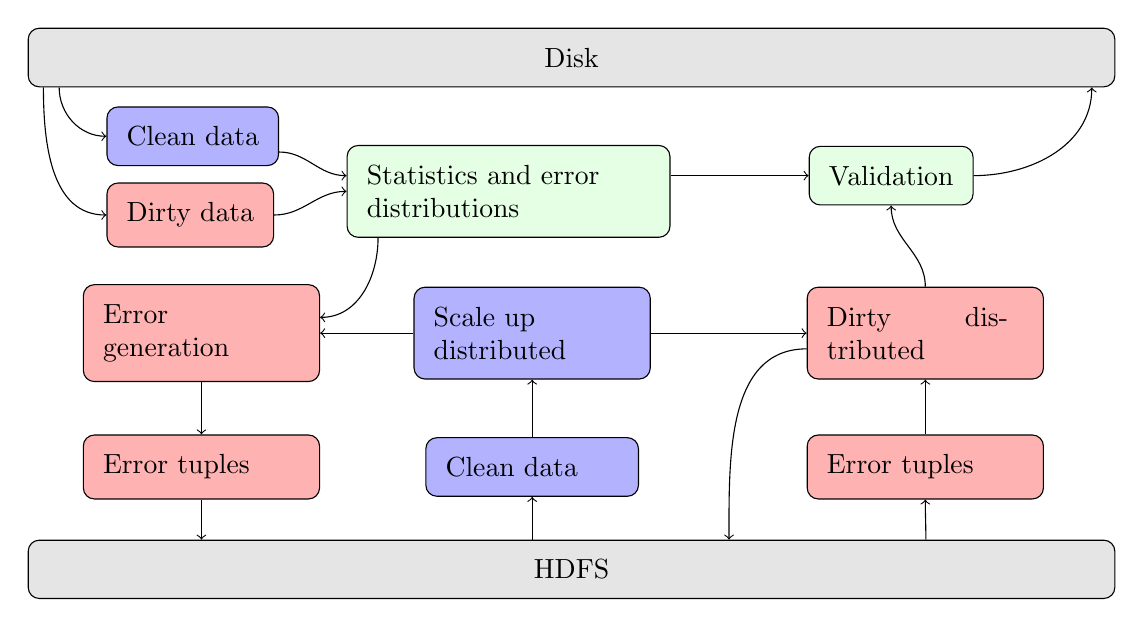
\begin{tikzpicture}[]
    \node[bb, text width=13.3cm, align = center, fill=black!10](disk){Disk};
    
    \node[bb, text width=13.3cm, align = center, fill=black!10] (hdfs) at ([yshift=-6.5cm] disk){HDFS};
    
    \node[bb, anchor = west, fill=blue!30] (clean) at ([yshift=-1.cm, xshift = 1cm] disk.west) {Clean data};
    \node[bb, anchor = west, fill=red!30] (dirty) at ([yshift=-2cm, xshift = 1cm] disk.west) {Dirty data};
    
    \node[bb, text width=2.2cm, fill=blue!30] (clean_dist) at ([yshift=-5.2cm, xshift = -0.5cm] disk) {Clean data};
    
    \node[bb, text width=3.6cm, fill=green!10] (stats) at ([yshift=-1.7cm, xshift = -0.8cm] disk) {Statistics and error distributions};
    
    \node[bb, text width=2.5cm, fill=blue!30] (scale_up) at ([yshift=-3.5cm, xshift = -0.5cm] disk) {Scale up \ \ \ \ \ \ \ \ \  distributed };
    
    \node[bb, text width=2.5cm, fill=red!30] (error_gen) at ([yshift=-3.5cm, xshift = -4.7cm] disk) {Error \ \ \ \ \ \ \ \ \ \ generation};
    \node[bb, text width=2.5cm, fill=red!30] (error_tuples) at ([yshift=-5.2cm, xshift = -4.7cm] disk) {Error tuples};
    
    % \node[bb, fill=red!30, text width=4.0cm, anchor = east] (errors) at ([yshift=-1.7cm,xshift= -0.8cm] disk.east) {Errors generation and introduction};
    
    \node[bb,  anchor=east, fill=green!10] (validation) at ([yshift=-1.5cm, xshift=-1.8cm] disk.east) {Validation};
    
    \node[bb,  anchor=east, fill=red!30, text width = 2.5cm] (dirty_dist) at ([yshift=-3.5cm, xshift=6cm] disk) {Dirty \ \ \ \ \ \ \ distributed};
    
    \node[bb, anchor=east, text width=2.5cm, fill=red!30] (error_tuples_out) at ([yshift=-5.2cm, xshift = 6cm] disk) {Error tuples};
    
    
    \draw[->] ([xshift=0.4cm]disk.south west) to[out = -90, in = 180] (clean);
    \draw[->] ([xshift=-0.5cm]hdfs.north) to[out = 90, in = -90] (clean_dist);
    \draw[->] ([xshift=0.0cm]clean_dist.north) to[out = 90, in = -90] (scale_up);
    \draw[->] ([xshift=0.2cm]disk.south west) to[out = -90, in = 180] (dirty);
    
    \draw[->] ([xshift=0.4cm, yshift=-0.0cm]stats.south west) to[out = -90, in = 0] ([yshift=0.2cm]error_gen.east);
    \draw[->] ([yshift=-0.0cm]scale_up.west) to[out = 180, in = 0] ([yshift=-0.0cm]error_gen.east);
    \draw[->] ([xshift=0.0cm]error_tuples.south) to[out = -90, in = 90] ([xshift=-4.7cm]hdfs.north);
    \draw[->] ([xshift=0.0cm]error_gen.south) to[out = -90, in = 90] ([xshift=0cm]error_tuples.north);
    
    % \draw[->] ([]clean.east) to[out = 0, in = 180] (scale_up);
    
    \draw[->] ([yshift=-0.2cm]clean.east) to[out = 0, in = 180] ([yshift=0.2cm] stats.west);
    
    \draw[->] ([]dirty.east) to[out = 0, in = 180] (stats);
    
    % \draw[->] ([]scale_up.east) to[out = 0, in = 180] (errors);
    
    % \draw[->] ([]stats.east) to[out = 0, in = -90] ([xshift=0.2cm]errors.south west);
    
    % \draw[->] ([]errors.east) to[out = 30, in = -90] ([xshift=-0.5cm]disk.south east);
    
    \draw[->] ([]validation.east) to[out = 0, in = -90] ([xshift=-0.3cm]disk.south east);
    
    % \draw[->] ([xshift=-0.8cm]errors.south) to[out = -90, in = 180] ([]validation.west);
    
    \draw[->] ([yshift=0.2cm]stats.east) to[out = 0, in = 180] ([yshift=-0.0cm]validation.west);
    
    \draw[->] ([xshift=4.5cm]hdfs.north) to[out = 90, in = -90] (error_tuples_out);
    
    \draw[->] ([xshift=0cm]error_tuples_out.north) to[out = 90, in = -90] (dirty_dist);
    
    \draw[->] ([xshift=0cm]scale_up.east) to[out = 0, in = 180] (dirty_dist.west);
    
    \draw[->] ([yshift=-0.2cm]dirty_dist.west) to[out = 180, in = 90] ([xshift=2cm]hdfs.north);
    
    \draw[->] ([yshift=0cm]dirty_dist.north) to[out = 90, in = -90] ([xshift=0cm]validation.south);
    
    \end{tikzpicture}
    
    \caption{\label{fig:data_gen_dist}Distributed data generator}
    
\end{figure}

% Checked with grammarly
\section{Validation of Results}

% To check results after generation such statistics as min, max, mean, variance, skew are compared. Additionally, missing values,  distinct values and outliers are checked. 
% To have history of modifications, after every transformation binary mask is stored and can be loaded if needed. Super mask with all modified cells is picked during the run time.

% univar statistics
% schema
% masking

To validate the data and to evaluate error generation a number statistics is computed before and after the data generation:
% TODO maybe table with stat and rule 
\begin{itemize}
    \item shape. 
    \item distinct values.
    \item functional dependencies.
    \item outliers.
    \item missing values.
    \item min, max and mode
    \item mean and variance.
    \item skewness and curtosis.
\end{itemize}

Dimensions and shape of the scaled erroneous data should correspond the original data and the scaling factor. 
Similarly, disctinct values remain the same unless they were corrupted for induvidual features.
Functional dependencies can be either given as an input, or discovered from the data. Importantly, after the scaling FDs should remain the same. Only after FDs corruption error, FDs change.
Outliers are computed by interquartile range (IQR) and are tracked with masks. Observation/row should have the same outlier mask before and after scaling since data is scaled by random sampling.
Missing values are traced similarly to the outliers. If cell contained a missing value before scaling or error generation, it should also contain it after.
\\
Data ranges are assumed to be same after scaling, but this property doesn't hold after the error generation. 
Mean, variance, skewness and curtosis should fluctuate within 20\%. 
This means that if originally feature was approximately symmetric (skeweness between -0.5 and 0.5), the skeweness of the symmetric should be within [-0.7, 0.7] interval.
\\
For easier error introduction and to assure that the feature type constraints are not violated, the schema of the original data is detected and preserved.
Schema detection is implemented by sampling the input dataset and extracting basic data types (e.g., integer, float, string). 
\\
To trace changes during the error introduction masks are computed as described in Chapter 3. Additionally, statistics of scaled data are modified.
% TODO 
\\In distributed setting, distinct values and other statistics are computed before partitioning. 


